\documentclass{article}
\usepackage[utf8]{inputenc}
\usepackage[english]{babel}

\usepackage{tikz}
\usetikzlibrary{graphs, positioning, arrows}

\usepackage{amssymb,latexsym,amsmath,amscd,amsthm, mathtools,stmaryrd, hyperref, enumitem, cleveref}

\theoremstyle{theorem}
\newtheorem{theorem}{Theorem}

\theoremstyle{definition}
\newtheorem{definition}{Definition}
\newtheorem{remark}{Remark}
\newtheorem{example}{Example}


%opening
\title{Supersingular Isogeny Diffie-Hellman}
\author{Valeriia Kulynych\\ Université de Toulon}

\begin{document}

\maketitle

\section{Supersingular Elliptic Curves}

\subsection{Various definitions}

Let $K$ be a field with algebraic closure $\bar{K}$.

\begin{definition}[Projective space]
	The \textit{projective space of dimension $n$}, denoted by $\mathbb{P}^n$ or $\mathbb{P}^n(\bar{K})$ is the set of all $(n+1)$-tuples
		\[ (x_0, \dots, x_n) \in \bar{K}^{n+1} \]
	such that $(x_0, dots, x_n) \neq (0, \dots, 0)$ taken modulo the equivalence relation 
		\[ (x_0, \dots, x_n) \sim (y_0, \dots, y_n) \]
	if and only in there exists $\lambda \in \bar{K}, \lambda \neq 0$ such that $x_i = \lambda y_i$ for all $i$ (Cf. \cite[I]{IsogenyCryptoDeFeo}).
\end{definition}


The equivalence class of a projective point $(x_0, \dots, x_n)$ is denoted by $[x_0, \dots, x_n]$. The set of $K$-rational points, denoted by $\mathbb{P}^n(K)$, is defined as 
	\[ \mathbb{P}^n(K) = \{ [x_0, \dots, x_n] \in \mathbb{P}^n | x_i \in K \ \text{for all} \ i \} \]

\begin{definition}[Elliptic curve] 
	An \textit{elliptic curve} is a pair $(E, O)$, where $E$ is a curve of genus 1 and $O \in E$. (We often just write $E$ for the elliptic curve, the point $O$ is being understood.) $E(K)$ is the subgroup of rational points over field $k$ on the curve $E$. The elliptic curve $E$ is defined over $K$, written $E/K$, if $E$ is defined over $K$ as a curve and $O \in E(K)$. (Cf. \cite[III, \S3]{Silverman}).
\end{definition}

Let $E$ be an elliptic curve given by a Weierstrass equation (see page \pageref{WE}). Remember that $E \subset \mathbb{P}^2$ consists of the points $P = (x, y)$ satisfying the Weierstrass equation together with the point $O = [0, 1, 0]$ at infinity. Let $L \subset \mathbb{P}^2$ be a line. Then since the equation has degree three, $L$ intersects $E$ at exactly 3 points, say $P, Q, R$. (Note if $L$ is tangent to $E$, then $P, Q, R$ may not be distinct. The fact that $L \cap E$ taken with multiplicities, consists of three points, is a special case of Bezout's theorem (Cf. \cite[I.7, Corollary 7.8]{Hartshorne}).

Define a composition law $\oplus$ on $E$ by the following rule.

\begin{definition}[Composition law]
	Let $P, Q \in E$, $L$ be the line connecting $P$ and $Q$ (tangent line to $E$ if $P = Q$), and $R$ be the third point of intersection of $L$ with $E$. Let $L'$ be the line connecting $R$ and $O$. Then $P \oplus Q$ is the point such that $L'$ intersects $E$ at $R, O \ \text{and} \ P \oplus Q$ (Cf. \cite[III, \S2]{Silverman}).
\end{definition}

Let $E$ be an elliptic curve defined over $K$. As $E$ with composition law $\oplus$ has an abelian group structure, then we can define subgroup of its rational points over the field $K$ and denote it $E(K)$. 

Now we assume that the characteristic of $K$ is $p > 0$.

	\begin{definition}[Supersingular elliptic curve] \label{ssedef1}
		For every $n$, we have a multiplication map 
		\[[n]: E \to E\]
		\[ P \mapsto \underbrace{P \oplus \cdots \oplus P}_{n \ \text{times}}. \]
		Its kernel is denoted by $E[n]$ and is called the $n$-torsion subgroup of $E$. Then one can show that for any $r \geq 1$:
		\[ E[p^r](\bar{K}) \simeq
			\begin{cases}
			{0} \\
			\mathbb{Z}/p^r\mathbb{Z}
		\end{cases} \]
		In the first case, $E$ is called \textit{supersingular}. Otherwise, it is called \textit{ordinary} (Cf. \cite[V, \S3, Theorem 3.1]{Silverman}).
	\end{definition}

For each integer $r \geq 1$ we consider the $p^r$-power Frobenius morphism (Cf. \cite[II, \S2]{Silverman}) given by  
	\[\phi_r: E \to E^{(p^r)}\]
	\[ [x_0, \dots, x_n] \mapsto [x_0^{p^r}, \dots, x_n^{p^r}] \]
Let $m = \mathrm{deg}\phi_r$. 
Then we consider the morphism
	\[\hat{\phi_r}: E^{(p^r)} \to E, \]
such that 
	\[ \hat{\phi_r} \circ \phi_r = [m], \]
where $[m]$ is $m$-multiplication map. Such $\hat{\phi_r}$ is called \textit{dual} of $p^r$-power Frobenius morphism (Cf. \cite[III, \S6, Theorem 6.1]{Silverman}). 

We remind that morphism $f: X \to Y$ is separable if $K(X)$ is a separable extension of $K(Y)$ (Cf. \cite[IV, 2]{Hartshorne}).

We remind the notion of separable extension. Let $F$ be a finite extension of $K$. We say that $F$ is separable over $K$ if $[F:K]_S = [F:K]$, where $[F:K]_S$ is a separable degree of $F$ over $K$. An element $\alpha$ algebraic over $K$ is said to be separable over $K$ if its minimal polynomial has no multiple roots.(Cf. \cite[V, \S4]{Lang}) Then one can show that $F$ is separable over $K$ if and only if each element of $F$ is sepable over $K$ (Cf. \cite[V, \S4, Theorem 4.3]{Lang}). Extensions which are not separable are called \textit{inseparable}.

A finite extension $K$ of field $k$ is \textit{purely inseparable} if for every $\alpha \in K$, $\alpha^{p^m} \in k$ for some $m \geq 0$ (Cf. \cite{PurelyInseparable}).
 
That brings us to another approach to define supersingular elliptic curve:
	\begin{definition}[Supersingular elliptic curve]
		An elliptic curve $E$ is supersingular if the map $\hat{\phi_r}$ is (purely) inseparable for one (all) $r \geq 1$ (Cf. \cite[V, \S3, Theorem 3.1]{Silverman}).
	\end{definition}

\begin{definition}[Weierstrass equation]\label{WE}
	An ellipric curve defined over $K$ is the locus in $\mathbb{P}^2$ of an equation
		\[ Y^2Z + a_1XYZ + a_3YZ^2 = X^3 + a_2X^2Z + a_4XZ^2 + a_6Z^3,  \]
	with $a_1,\dots, a_6 \in \bar{K}$. This equation is called a \textit{Weierstrass equation} (Cf. \cite[III, \S1]{Silverman}).
\end{definition} 

To ease notation, we will usually write the Weierstrass equation for our elliptic curve using non-homogeneous coordinates $x = X/Z$ and $y = Y/Z$, 
	\[ E: y^2 + a_1xy + a_3y = x^3 +a_2x^2 + a_4x +a_6, \]
always remembering that there is the extra point $O = [0, 1, 0]$ out at infinity. 

If $\mathrm{char}(\bar{K}) \neq 2$, then we can simplify the equation by completing the square. Replacing $y$ by $\frac{1}{2}(y - a_1x - a_3)$ gives an equation of the form
	\[E: y^2 = 4x^3 + b_2x^2 +2b_4x + b_6, \]
where
	\[b_2 = a_1^2 + 4a_2,\]
	\[b_4 = 2a_4 + a_1a_3,\]
	\[b_6 = a_3^2 + 4a_6.\]
We also define quantities
	\[b_8 = a_1^2a_6 + 4a_2a_6 - a_1a_3a_4 + a_2a_3^2 - a_4^2,\]
	\[c_4 = b_2^2 - 24b_4, \]
	\[c_6 = b_2^3 + 36b_2b_4 - 216b_6,\]
	\[\Delta = -b_2^2b_8 - 8b_4^3 - 27b_6^2 + 9b_2b_4b_6, \]
	\[j = c_4^2/\Delta.\]
%If further we have $\mathrm{char}(\bar{K}) \neq 2, 3$, then replacing $(x, y)$ by $(\frac{x - 3b_2}{36}, \frac{y}{216})$ eliminates the $x^2$ term, yielding the simpler equation
%	\[E: y^2 = x^3 - 27c_4x - 54c_6. \] 
	
The quantity $\Delta$ given above is called the \textit{discriminant} of the Weierstrass equation, $j$ is called the \textit{$j$-invariant} \label{j-invariant} of the elliptic curve $E$. Now we can given another one definition of a supersingular elliptic curve:
	\begin{definition}[Supersingular elliptic curve]
		If the map $[p]: E \to E$ is purely inseparable and $j(E) \in \mathbb{F}_{p^2}$ then the curve $E$ is called supersingular (Cf. \cite[V, \S3, Theorem 3.1]{Silverman}).
	\end{definition}


For the next definition of supersingular elliptic curve, we need to introduce the following notions. 

\begin{definition}[Order]
	Let $\mathcal{K}$ be a (not necessarily commutative) algebra (i.e. vector space equipped with a bilinear product), finitely generated over $\mathbb{Q}$. An \textit{order} $\mathcal{R}$ of $\mathcal{K}$ is a subring of $\mathcal{K}$ which is finitely generated as $\mathbb{Z}$-module (i.e. as an abelian group) and which satisfies $\mathcal{R} \otimes \mathbb{Q} = \mathcal{K}$, where $\otimes$ is the tensor product (Cf. \cite[III, \S9]{Silverman}).
\end{definition}

\begin{definition}[Quaternion algebra]
	A \textit{quaternion algebra} is an algebra of the form
	\[ \mathcal{K} = \mathbb{Q} +\mathbb{Q}\alpha + \mathbb{Q}\beta +\mathbb{Q}\alpha\beta \]
	with the multiplication rules
	\[ \alpha^2, \beta^2 \in \mathbb{Q}, \quad \alpha^2 < 0, \quad \beta^2 < 0, \quad \beta\alpha = - \alpha\beta. \] (Cf. \cite[III, \S9]{Silverman}).
\end{definition}

\begin{definition}[Supersingular elliptic curve]
	An elliptic curve $E$ is supersingular if the endomorphism		ring $\mathrm{End}_{\bar{K}}(E)$ is an order in a quaternion algebra (Cf. \cite[V, \S3, Theorem 3.1]{Silverman}).
\end{definition}

\begin{remark}
 	The endomorphism ring of an elliptic curve is either $\mathbb{Z}$ (if $p = 0$), an order in an imaginary quadratic number field (a number field of the form $\mathbb{Q}[\sqrt{-D}]$ for some $D > 0$), or an order in a quaternion algebra (Cf. \cite[III, \S, Corollary 9.4]{Silverman}).  
\end{remark}

Another way to define supersingular elliptic curve is based on a notion of a formal group.

Let $R$ be a ring of characteristic $p > 0$.
\begin{definition}[Formal group]
	 A \textit{(one-parameter commutative) formal group $\mathcal{F}$ defined over $R$} is a power series $F(X, Y) \in R\llbracket X, Y \rrbracket $ satisfying:
		\begin{enumerate}
			\item $F(X, Y) = X + Y + \ \text{(terms of degree} \ \geq 2)$.
			\item $F(X, F(Y, Z)) = F(F(X, Y), Z)$ (associativity).
			\item $F(X, Y) = F(Y, X)$ (commutativity).
			\item There is unique power series $i(T) \in R\llbracket T \rrbracket$ such that $F(T, i(T)) = 0$ (inverse).
			\item $F(X, 0) = 0$ and $F(0, Y) = Y$.
		\end{enumerate} \cite[IV, \S2]{Silverman}.
\end{definition}

We call $F(X,Y)$ the \textit{formal group law of $\mathcal{F}$}.
 
Returning now to formal power series, we look for the power series formally giving the addition law on E. Thus let $z_1, z_2$ be independent indeterminates, and let 
	\[w_i = w(z_i) = z_i^3(1 + A_1z_i + A_2z_i^2 + \cdots) \in \mathbb{Z}[a_1, \dots, a_6]\llbracket z_i \rrbracket,\]
where $A_i \in \mathbb{Z}[a_1, \dots, a_6]$, for $i = 1, 2$. In the $(z, w)$-plane, the line connecting $(z_1, w_1)$ to $(z_2, w_2)$ has slope
	\[ \lambda = \lambda(z_1, z_2) = \frac{w_2 - w_1}{z_2 - z_1} = \sum_{n = 3}^{\infty} A_n\frac{z_2^n -z_1^n}{z_2 - z_1} \in \mathbb{Z}[a_1, \dots, a_6]\llbracket z_1, z_2 \rrbracket. \]
Letting
	\[v = v(z_1, z_2) = w_1 - \lambda z_1 \in \mathbb{Z}[a_1, \dots, a_6]\llbracket z_1, z_2 \rrbracket, \]
the connecting line has equation $w = \lambda z +v$. Substituting this into the Weierstrass equation gives a cubic in $z$, two of whose roots are $z_1$ and $z_2$. Looking at the quadratic term, we see that the third $z_3$ can be expressed as a power series in $z_1$ and $z_2$:
	\[z_3 = z_3(z_1, z_2) =\]
	\[= -z_1 -z_2 + \frac{a_1\lambda + a_3\lambda^2 -a_2v - 2a_4\lambda v - 3a_6\lambda^2v}{1 + a_2\lambda + a_4\lambda^2 + a_6\lambda^3}\]
	\[\in \mathbb{Z}[a_1, \dots, a_6]\llbracket z_1, z_2 \rrbracket.\]
For the group law on $E$, the points $(z_1, w_1), (z_2, w_2), (z_3, w_3)$ add up to zero. Thus to add the first two, we need the formula for the inverse. In the $(x, y)$-plane, the inverse of $(x, y)$ is $(x, -y -a_1x - a_3)$. Hence the inverse of $(z, w)$ will have $z$-coordinate ($z = -x/y$)
	\[ i(z) = \frac{x(z)}{y(z) + a_1x(z) + a_3} = \frac{z^{-2} - a_1z^{-1} - \dots}{-z^{-3} + 2a_1z^{-2} + \dots } \]
This gives the formal additional law 
	\[F(z_1, z_2) = i(z_3(z_1, z_2)) = \]
	\[= z_1 + z_2 - a_1z_1z_2 - a_2(z_1^2z_2 + z_1z_2^2) - (2a_3z_1^3z_2 - (a_1a_2 - 3a_3)z_1^2z_2^2 + 2a_3z_1z_2^3) + \dots \]
	\[\in \mathbb{Z}[a_1, \dots, a_6] \llbracket z_1, z_2 \rrbracket. \]
Let $E$ be an elliptic curve given by a Weierstrass equation with coefficients in $R$. The \textit{formal group associated to $E$}, denoted $\hat{E}$, is given by the power series $F(z_1, z_2)$ described above.
 
\begin{definition}[Height of homomorphism; height of formal group]
	Let $\mathcal{F}, \mathcal{G}$ defined over $R$ be formal groups and $f: \mathcal{F} \to \mathcal{G}$ a homomorphism defined over $R$. The \textit{height of $f$}, denoted $ht(f)$, is the largest integer $h$ such that 
		\[f(T) = g(T^{p^h}) \]
	for some power series $g(T) \in R \llbracket T \rrbracket$. (If $f = 0$, then $ht(f) = \infty$.) The \textit{height of $\mathcal{F}$}, denoted $ht(\mathcal{F})$, is the height of the multiplication by $p$ map $[p]: \mathcal{F} \to \mathcal{F}$ \cite[IV, \S7]{Silverman}.
\end{definition}

	\begin{definition}[Supersingular elliptic curve]
		If the formal group $\hat{E}/K$ associated to $E$ has height 2, then $E$ is supersingular \cite[V, \S3, Theorem 3.1]{Silverman}. 
	\end{definition}

For the next approach to define supersingular curve we introduce an important invariant of elliptic curve $E$ defined over a perfect field $K$ of characteristic $p > 0$.

Let $F: E \to E$ be the Frobenius morphism. Then F induces a map:
	\[ F^{\ast}: H^1(E, \mathcal{O}_E) \to H^1(E, \mathcal{O}_E)  \]
on cohomology. This map is not linear, but it is \textit{$p$-linear}, namely $F^{\ast}(\lambda a) = \lambda^pF^{\ast}(a)$ for all $\lambda \in K, a \in H^1(E, O_E)$. Since $E$ is elliptic, $H^1(E, O_E)$ is a one-dimensional vector space. Thus, since $K$ is perfect, the map $F^{\ast}$ is either 0 or bijective.
For more information on cohomology see \cite[III]{Hartshorne}.
	\begin{definition}[Hasse invariant, Supersingular elliptic curve]
		If $F^{\ast} = 0$, we say that $E$ has \textit{Hasse invariant $0$} or that $E$ is \textit{supersingular}; otherwise we say that $E$ has \textit{Hasse invariant 1} \cite[IV, 4]{Hartshorne}.
	\end{definition}

The next theorem also could be used as a definition.
	\begin{theorem} 
		An elliptic curve $E/\mathbb{F}_q$ is supersingular if and only if $\mathrm{tr}\phi_E \cong 0 \mathrm{mod} p$, where $\phi_E$ is the Frobenius morphism (Cf. \cite[Lecture 14]{SutherlandEllipticCurves}).
	\end{theorem}
		\begin{proof}
			We first suppose that $E$ is supersingular and assume $q = p^n$ so that $\phi_E = \phi^n$. Then $\mathrm{ker}[p] = \mathrm{ker}\phi\hat{\phi}$ is trivial, and therefore $\mathrm{ker}\hat{\phi}$ is trivial. Thus $\hat{\phi}$ is inseparable, since it has degree $p > 1$. The isogeny (see \pageref{isogeny}) $\hat{\phi}^n = \hat{\phi^n} = \hat{\phi}_E$ is also inseparable,as is $\phi_E$, so $\mathrm{tr}\phi_E = \phi_E + \hat{\phi}_E$ is a sum of inseparable endomorphisms, hence inseparable (here we are viewing the integer $\mathrm{tr}\phi$ as an endomorphism). Therefore $\mathrm{deg}(\mathrm{tr}\phi_E) = (\mathrm{tr}\phi_E)^2$ is divisible by $p$, so $\mathrm{tr}\phi_E \cong 0 \mathrm{mod} p.$
			
			Conversely, if $\mathrm{tr}\phi_E \cong 0 \mathrm{mod} p$, then $p$ divides $\mathrm{deg}(\mathrm{tr}\phi_E) = (\mathrm{tr}\phi_E)^2$ and $\mathrm{tr}\phi_E$ is inseparable, as is $\hat{\phi}_E = \mathrm{tr}\phi_E - \phi_E$. This means that $\hat{\phi}^n$ and therefore $\hat{\phi}$ is inseparable. So $\mathrm{ker}\hat{\phi}$ is trivial, since it has prime degree $p$, and the same is true for $\phi$. Thus the kernel of $[p] = \hat{\phi}\phi$ is trivial and $E$ is supersingular.
		\end{proof}
		

When $q=p$ is a prime greater than 3 this is equivalent to having the trace of Frobenius morphism equal to zero; this does not hold for $p = 2 \ \text{or} \ 3$.

 \subsection{Examples}

In this section we are going to give some examples of supersingular curves.

Using definitions given in previous section may not always be a convenient way to identify a supersingular curves. But from those equivalent definitions we see thath up to isomorphism, there are only finitely many elliptic curves with Hasse invariant 0, since each has $j$-invariant in $\mathbb{F}_{p^2}$. For $p = 2$, once can easily check that the only one supersingular elliptic curve is 
	\[ E: y^2 + y = x^3. \]
For $p > 2$, the following theorem gives a simple criterion for determining whether an elliptic curve is supersingular.

\begin{theorem} \label{thm1}
	Let $K$ be finite field of characteristic $p > 2$.
		\begin{enumerate}[label = (\alph*)]
			\item Let $E/K$ be an elliptic curve with Weierstrass equation 
					\[ E: y^2 = f(x) \]
				where $f(x) \in K[x]$ is a cubic polynomial with distinct roots (in $\bar{K}$). Then $E$ is supersingular if and only if the coefficient of $x^{p - 1}$ in $f(x)^{(p - 1)/2}$ is zero.
			
			\item  Let $m = (p - 1)/2$, and define a polynomial
					\[H_p(t) = \sum_{i = 0}^{m} \binom{m}{i}^2t^i. \]
				Let $\lambda \in \bar{K}$, $\lambda \neq 0, 1$. Then the elliptic curve
					\[E: y^2 = x(x - 1)(x - \lambda)  \]
				is supersingular if and only if $H_p(\lambda) = 0$.
			
			\item The polynomial $H_p(t)$ has distinct roots in $\bar{K}$. Up to isomorphism, there are exactly
					\[ [\frac{p}{12}] + \varepsilon_p \]
				supersingular elliptic curves in characteristic $p$, where $\varepsilon_3 = 1$, and for $p \geq 5$,
					\[\varepsilon_p = 0, 1, 1, 2 \quad \textrm{if} \quad p \cong 1, 5, 7, 11 (\mathrm{mod}12). \]
			(Cf. \cite[V, \S4, Theorem 4.1]{Silverman})
		\end{enumerate}
\end{theorem}

\begin{example}
	For which primes $p \geq 5$ is the elliptic curve
		\[E:  y^2 = x^3 + 1\]
	supersingular?
	
	Notice this curve has $j(E) = 0$. From the criterion of \cref{thm1}(a), we must compute the coefficient of $x^{p-1}$ in $(x^3 + 1)^{(p-1)/2}$. If $p \cong 2 \mathrm{mod} 3$, then there is no $x^{p-1}$ term, so $E$ is supersingular; while if $p \cong 1 \mathrm{mod} 3$, then the coefficients is $\binom{(p-1)/2}{(p-1)/3}$, which is non-zero modulo $p$, so in this case $E$ is ordinary.
\end{example}

\begin{example}
	Similary we compute for which primes $p \geq 3$ the $j = 1728$ elliptic curve
		\[E: y^2 = x^3 + x \]
	is supersingular.
	
	This is determined by the coefficient of $x^{(p-1)/2}$ in $(x^2 + 1)^{(p-1)/2}$, which equals $0$ if $p \cong 3 \mathrm{mod} 4$ and $\binom{(p-1)/2}{(p-1)/4}$ if $p \cong 1 \mathrm{mod} 4$. Hence $E$ is supersingular if $p \cong 3 \mathrm{mod} 4$ and ordinary if $p \cong 1 \mathrm{mod} 4$.
\end{example}

\begin{example}
	Let $E$ be given by the equation 
		\[E: y^2 + y = x^3 -x^2 -10x - 20,\]
	so $j(E) = -\frac{2^{12}31^3}{11^5}$. Then by using the criterion of \cref{thm1} (a) directly one finds that the only primes $p < 100$ for which $E$ is supersingular in characteristic $p$ are $p = 19$ and $p = 29$. (D. H. Lehmer has calculated that there are exactly $27$ primes $p < 31500$ for which this $E$ is supersingular.) 
\end{example}


\section{Isogeny Graphs}

We start this section with a notion of isogeny.
	\begin{definition} \label{isogeny}
		Let $E_1$ and $E_2$ be elliptic curves defined over a finite field $\mathbb{F}_q$ of characteristic $p$. An \textit{isogeny} $\phi: E_1 \to E_2$ defined over $\mathbb{F}_q$ is a non-constant morphism that maps the identity into the identity (and this a is group homomorphism) (Cf. \cite[2.1]{HardEasyProbs}).
	\end{definition}
Two elliptic curves $E_1$ and $E_2$ defined over $\mathbb{F}_q$ are said to be \textit{isogenous} over $\mathbb{F}_q$ if there exists an isgony $\phi: E_1 \to E_2$ defined over $\mathbb{F}_q$.

\begin{theorem}[Sato-Tate]
	Two elliptic curves $E_1$ and $E_2$ are isogenous over $\mathbb{F}_q$ if and only if $\#E_1(\mathbb{F}_q) = \#E_2(\mathbb{F}_q)$ (Cf. \cite[Theorem 13]{IsogenyCryptoDeFeo}). 
\end{theorem}  

The degree of an isogeny $\phi$ is the degree of $\phi$ as a morphism. An isogeny of degree $\ell$ is called $\ell$-isogeny. 

Curves in the same isogeny class are either all supersingular or all ordinary.

%For prime $\ell \not| p$, we have $E[\ell] \simeq \mathbb{Z}/\ell\mathbb{Z} \oplus \mathbb{Z}/\ell\mathbb{Z}$ \cite[2]{TowardsQuantumRes}.

%Supersingular curves are all defined over $\mathbb{F}_{p^2}$, and for every prime $\ell \not| p$, there exist $\ell + 1$ isogenies (counting multiplicities) of degree $\ell$ originating from any given such supersingular curve. An isogeny can be identified with its kernel. Given a subgroup $G$ of $E$, we can use Velu's formulas \cite[Proposition 39]{IsogenyCryptoDeFeo} to compute an isogeny $\phi: E_1 \to E_2$ with kernel $G$ and such that $E_2 \simeq E_1/G$. 

For each isogeny $\phi: E_1 \to E_2$, there is a unique isogeny $\hat{\phi}: E_2 \to E_1$ which is called the \textit{dual isogeny} of $\phi$, satisfying $\phi\hat{\phi} = \hat{\phi}\phi = [\mathrm{deg}\phi]$. 

If we have two isogenies $\phi: E_1 \to E_2$ and $\phi': E_2 \to E_1$ such that $\phi\phi'$ and $\phi'\phi$ are the identity in their respective curves, we say that $\phi$, $\phi'$ are \textit{isomorphisms}, and that $E$, $E'$ are \textit{isomorphic}. Isomorphism classes of elliptic curves over $\mathbb{F}_q$ can be labeled with their $j$-invariants (see page \pageref{j-invariant}). In this paper we write $j(E)$ for the $j$-invariant of $E$. By convention given a $j$-invariant $j \neq 0, 1728$, we write $E(j)$ for the curve defined by the equation 
	\[y^2 = x^3 + \frac{3j}{1728 - j}x + \frac{2j}{1728 - j}. \]
We also write $E(0)$ and $E(1728)$ for the curves with equations
	\[y^2 = x^3 + 1 \quad \text{and} \quad y^2 = x^3 +x \]
respectively.

	\begin{definition}[Isogeny graph]
		Let $E$ be an elliptic curve over a field $K$ of characteristic $p$. Let $S \subseteq \mathbb{N}$ be a finite set of primes. Define
			\[X_{E, K, S} \]
		to be the graph with vertex set being the $K$-isogeny class of $E$. Vertices are typically labelled by $j(E)$, though we also speak of "the vertex $E$". There is an edge $(j(E_1), j(E_2))$ labelled by $\ell$ for ezch equivalence class of $\ell$-isogenies from $E_1$ to $E_2$ defined over $K$ for some $\ell \in S$. We usually treat this as an undirected graph, since for every $\ell$-isogeny $\phi: E_1 \to E_2$ there is a dual isogeny $\hat{\phi}: E_2 \to E_1$ of degree $\ell$ (Cf. \cite[25.2]{Galbraith-PKC}). 
	\end{definition}

\subsection{Supersingular isogeny graph}

For the supersingular isogey graph we work over $\bar{\mathbb{F}}_p$. The graph is finite. Indeed, \cref{thm1} (c) implies $\frac{p}{12} - 1 < \#X_{E, \bar{\mathbb{F}}_p, S} < \frac{p}{12} + 2$. Note that it suffices to consider elliptic curves defined over $\mathbb{F}_{p^2}$ (although the isogenies between them are over $\bar{\mathbb{F}}_p$ in genereal).

In contrast to the ordinary case , the supersingular graph is always connected using isogenies of any fixed degree (Cf. \cite[2.4]{Mestre}).

\begin{theorem}
	Let $p$ be a prime and let $E$ and $\tilde{E}$ be supersingular elliptic curves over $\bar{\mathbb{F}}_p$. Let $\ell$ be a prime different from $p$. Then there is an isogeny from $E$ to $\tilde{E}$ over $\bar{\mathbb{F}}_p$ whose degree is a power of $\ell$ (Cf. \cite[2.4]{Mestre}).
\end{theorem}

Hence, one can choose any prime $\ell$ and consider the $\ell$-isogeny graphh $X_{e,\bar{\mathbb{F}}_p, {\ell}}$ on supersingular curves over $\bar{\mathbb{F}}_p$. It follows that the graph is $(\ell + 1)$-regular and connected.

Now we will give some examples of supersingular isogeny graphs.

\begin{figure}[h]
\begin{center}
	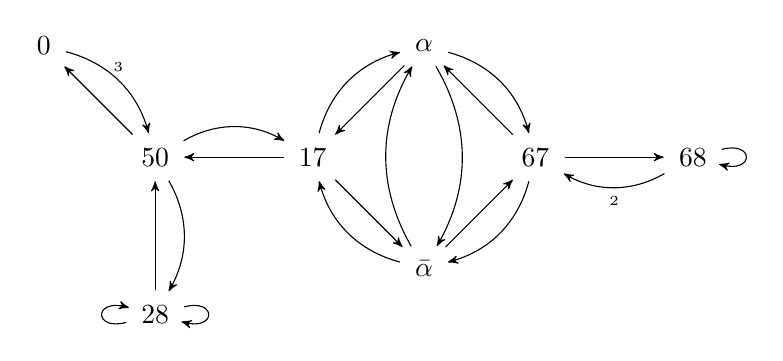
\begin{tikzpicture}[->, shorten >=2pt, shorten <=2pt, >=stealth', node distance = 2cm]

		\node (1) {$17$};
		\node (2) [above right of=1] {$\alpha$};
		\node (3) [below right of=1] {$\bar{\alpha}$};
		\node (4) [below right of=2] {$67$};
		\node (5) [right of=4] {$68$};
		\node (6) [left of=1] {$50$};
		\node (7) [below of=6] {$28$};
		\node (8) [above left of=6] {$0$};

			\path
				(1) edge [bend left] (2)
				(1) edge (3)
				(1) edge (6)
				
				(2) edge (1)
				(2) edge [bend left] (3)
				(2) edge [bend left] (4)
				
				(3) edge [bend left] (1)
				(3) edge [bend left] (2)
				(3) edge (4)
				
				(4) edge (2)
				(4) edge [bend left] (3)
				(4) edge (5)
				
				(5) edge [bend left] node[below]{\tiny{$2$}} (4)
				(5) edge [loop right] (5)
				
				(6) edge [bend left] (1)
				(6) edge [bend left] (7)
				(6) edge (8)
				
				(7) edge (6)
				(7) edge [loop left] (7)
				(7) edge [loop right] (7)
				
				(8) edge [bend left] node[above]{\tiny{$3$}} (6);
  
\end{tikzpicture}
\end{center}
\caption{Supersingular Isogeny Graph $X_{\bar{\mathbb{F}}_{83}, 2}$}\label{SIG83.figure}
\end{figure}

\begin{thebibliography}{}
	\bibitem{PurelyInseparable} Lindsay N. Childs. \textit{Purely Inseparable Field Extension}. \url{http://www.math.cornell.edu/~dkmiller/galmod/Childs_purely-inseparable.pdf}
	
	\bibitem{IsogenyCryptoDeFeo} Luca De Feo. \textit{Mathematics of isogeny based cryptography}, 2017.
	
	\bibitem{TowardsQuantumRes} Luca De Feo, David Jao, Jerome Plut. \textit{Towards Quantum-Resistant Cryptosystems From Supersingular Elliptic Curve Isogenies}, Journal of Mathematical Cryptology, 2014, 8 (3), pp. 209-247. \url{https://eprint.iacr.org/2011/506.pdf}
	
	\bibitem{Galbraith-PKC} Steven D. Galbraith. \textit{Mathematics of Public Key Cryptography}. Cambridge University Press, 2012.
	
	\bibitem{Hartshorne} Robin Hartshorne. \textit{Algebraic Geometry}, volume 52 of \textit{Graduate Texts in Mathematics}. Springler, New-York, 1977.
	
	\bibitem{Lang} Serge Lang. \textit{Algebra}, volume 211 of \textit{Graduate Texts in Mathematics}. Springer-Verlag, New York, 2002.

	\bibitem{Mestre} J-F Mestre. \textit{La methode des graphes. Exemples et applications}, 2004.
	
	\bibitem{HardEasyProbs} Christophe Petit, Kristin Lauter. \textit{Hard and Easy Problems for Supersingular Isogeny Graphs}. 2018
	
	\bibitem{Silverman} Joseph H. Silverman. \textit{The arithmetic of elliptic curves}, volume 106 of \textit{Graduate Texts in Mathematics}. Springer-Verlag, New York, 1992.

	\bibitem{SutherlandEllipticCurves} Andrew V. Sutherland. \textit{  Elliptic Curves (18.783)}, Lecture Notes, Spring 2015, full course is available on \url{http://dspace.mit.edu/handle/1721.1/111949#files-area}
	
	
\end{thebibliography}

\end{document}

